\documentclass[border=4pt]{standalone}
\usepackage{tikz}
\usetikzlibrary{arrows.meta,bending}
\begin{document}
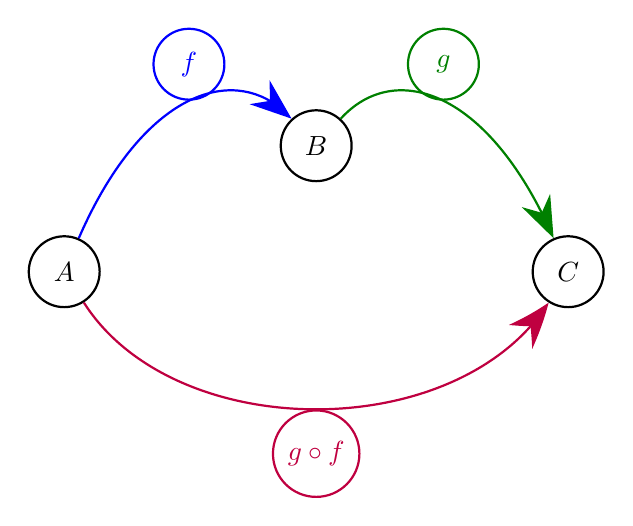
\begin{tikzpicture}[every node/.style={circle,draw,minimum size=9mm},line width=.8pt]
  \node (A) at (0,0) {$A$};
  \node (B) at (3.2,1.6) {$B$};
  \node (C) at (6.4,0) {$C$};

  \draw[blue,-{Stealth[length=15pt,flex]}]
    (A) .. controls (1.0,2.3) and (2.2,2.7) .. (B)
    node[midway,above] {$f$};
  \draw[green!50!black,-{Stealth[length=15pt,flex'=.65]}]
    (B) .. controls (4.2,2.7) and (5.4,2.3) .. (C)
    node[midway,above] {$g$};
  \draw[purple,-{Stealth[length=16pt,bend]}]
    (A) .. controls (1.4,-2.2) and (5.0,-2.2) .. (C)
    node[midway,below] {$g\circ f$};
\end{tikzpicture}
\end{document}
